\section{DISCUSSION}

\subsection{Explain the change in air when traveling through the aerodynamic tube based on humidity}

The theoretical change in air state across the aerodynamic tube is illustrated in Figure \ref{fig:theory_diagram}.

\begin{figure}[H]
    \centering
    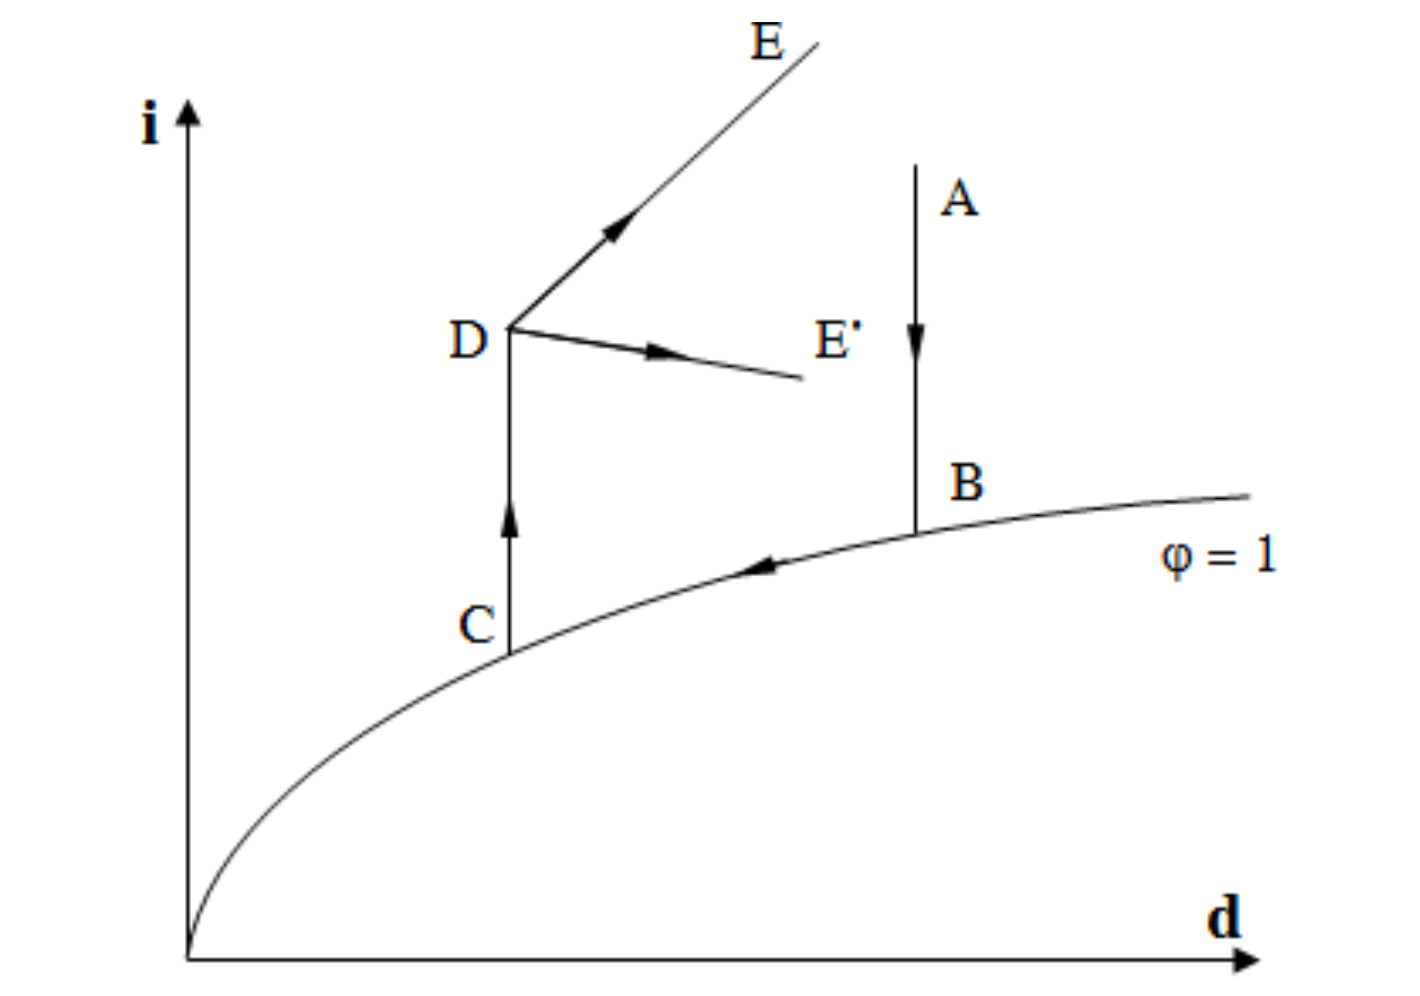
\includegraphics[width=0.75\linewidth]{Images/figure8.png}
    \caption{The diagram of the change in air when traveling through the aerodynamic tube in theory.}
    \label{fig:theory_diagram}
\end{figure}

\begin{itemize}
    \item \textbf{Through the cooler (lines AB and BC):} The change in the states of the air is represented by two straight lines AB and BC.
    \begin{itemize}
        \item In the \textit{early stage} of cooling (AB): The absolute humidity $d$ of the air remains unchanged (due to unchanged water content). Air temperature gradually decreases to the dew point temperature. Relative humidity $\varphi$ increases up to saturated state $\varphi = 1$. At dew point temperature B, corresponding to saturated state, the water begins to condense.
        \item In the \textit{later stage} of cooling (BC): The relative humidity $\varphi$ of the air remains unchanged and equals to 1, since the air is now saturated. As the air continues being cooled, the temperature continues decreasing. Absolute humidity $d$ of the air decreases as the condensed water makes the water content in humid air decrease.
    \end{itemize}

    \item \textbf{Through the dryer (line CD):} The absolute humidity $d$ of the air remains unchanged (due to unchanged water content) and the temperature of the air gradually increases. Relative humidity $\varphi$ gradually decreases.

    \item \textbf{Through the steam nozzle (line DE or DE'):}
    \begin{itemize}
        \item If using \textit{saturated steam}: the change in state of air is represented by the line DE. The absolute humidity $d$ increases as the air receives moisture. Enthalpy $I$ also increases as the air receives heat from saturated steam.
        \item If using \textit{superheated steam}: the change in state of air is represented by a straight line between DE and DE'. The more superheated the water is, the closer that line is to DE'. The absolute humidity $d$ increases. Enthalpy $I$ also increases but the increasing amount is smaller than when using saturated steam.
    \end{itemize}
\end{itemize}

\subsection{Explain why you can determine the humidity of the air through the dry bulb and wet bulb temperature}

\textbf{Dry bulb temperature:} The temperature of the gas mixture determined by the normal thermometer. The dry bulb temperature is also the temperature of the air because the mercury directly contacts with the air.

\textbf{Wet bulb temperature} is the steady temperature achieved when a very small amount of water evaporates into an unsaturated air mixture under adiabatic conditions. The wet bulb temperature is measured by a conventional thermometer whose mercury bulb is covered with a wet cloth. The dryer the air is or the smaller its relative humidity $\varphi$ is, the more water evaporates and the more heat surrounding air will lose; therefore, the lower wet bulb temperature is. When $\varphi = 0$, the difference between wet and dry bulb temperature is maximum. When $\varphi = 100\%$, the water cannot evaporate, so wet bulb temperature equals dry bulb temperature.

\vspace{0.3cm}
\noindent The relative humidity $\varphi$ of the air can be derived from the wet and dry bulb temperatures using the following derivation. Let $q_1$ be the heat that the air supplies to the wet bulb and $q_2$ be the heat consumed by evaporation:
\begin{equation*}
    q_1 = q_2
\end{equation*}
By heat transfer theory:
\begin{equation*}
    q_1 = \alpha (t_{dry} - t_{wet}), \quad q_2 = q_m \cdot r
\end{equation*}
Evaporation intensity $q_m$ (Dalton formula):
\begin{equation*}
    q_m = \alpha_m (p_m - p_a) \cdot \frac{1.013}{B}
\end{equation*}
Combining the above, we arrive at:
\begin{equation*}
    p_m - p_a = A \cdot B \cdot (t_{dry} - t_{wet})
\end{equation*}
where $A = \frac{\alpha}{\alpha_m \cdot 1.013 \cdot r}$ is the psychrometer factor. For $v < 0.5$ m/s, $A = 66 \times 10^{-5}$. Using $p_a = \varphi \cdot p_b$:
\begin{equation*}
    \varphi = \frac{p_m}{p_b} - \frac{A \cdot B}{p_b}(t_{dry} - t_{wet}) \tag{6}
\end{equation*}
where $p_m$ and $p_b$ are saturation pressures corresponding to wet bulb and dry bulb temperatures respectively.

Using the $I$-$d$ diagram one can also determine air state graphically:
\begin{enumerate}
    \item Draw a vertical line through $t_{wet}$, intersecting $\varphi = 1$ at point A.
    \item Draw a line through A parallel to $I = \text{const}$, intersecting the $t_{dry}$ line at point B.
    \item B is the state point of the air.
\end{enumerate}

\begin{figure}[H]
    \centering
    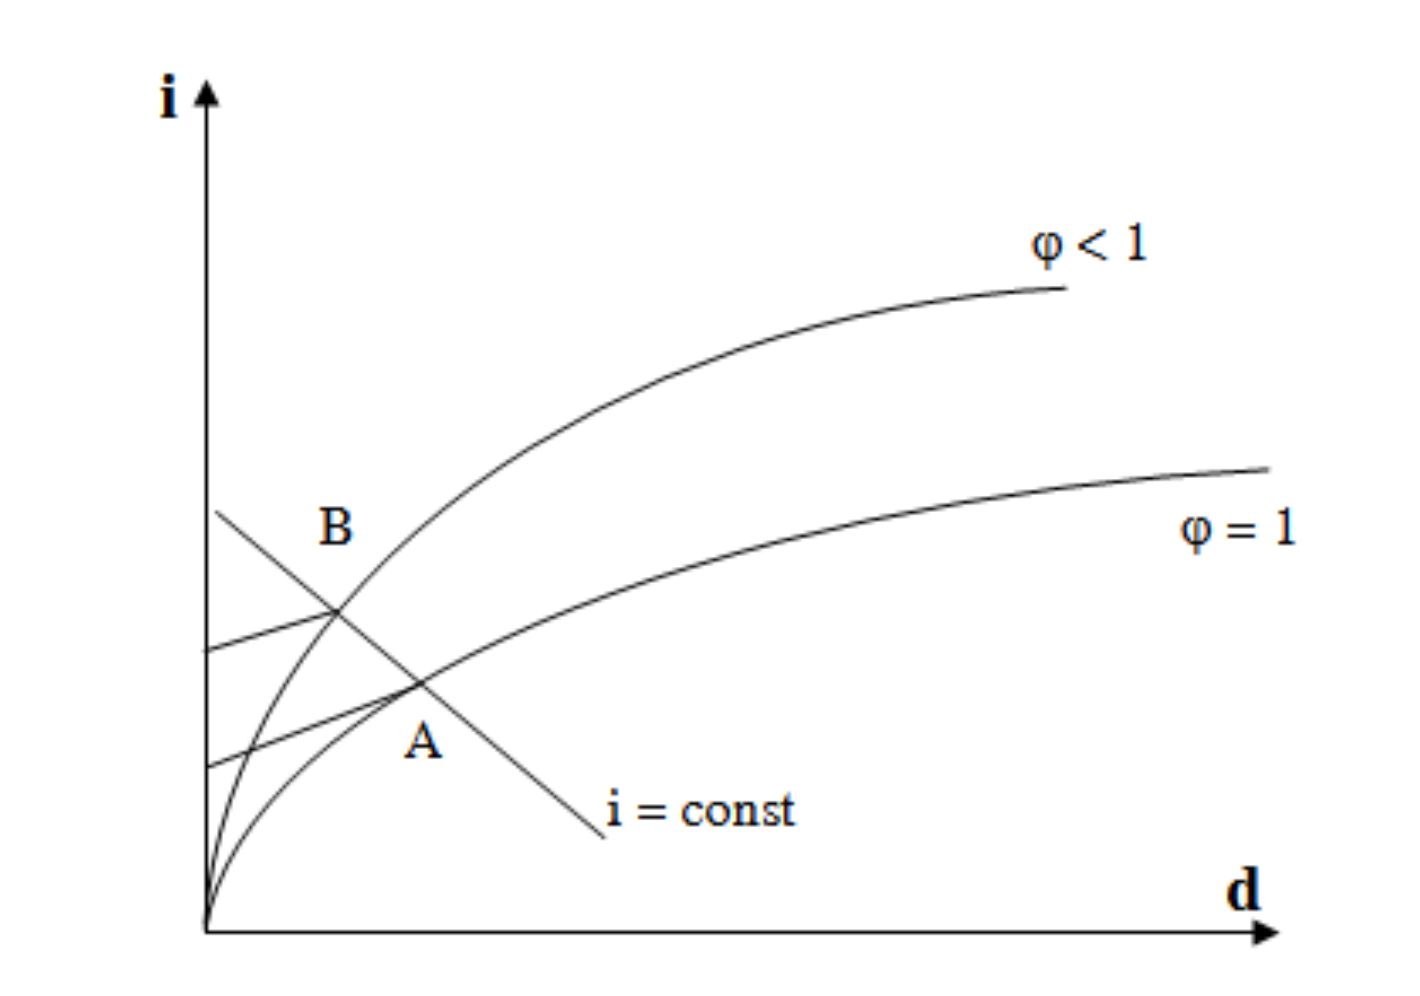
\includegraphics[width=0.65\linewidth]{Images/figure9.png}
    \caption{Way to determine humidity of the air using $I$-$d$ diagram, knowing wet bulb and dry bulb temperature.}
    \label{fig:id_humidity}
\end{figure}

\subsection{Comparisons between process in theory and practice (I-d diagram)}

The practical change in air state across the aerodynamic tube generally follows the same trend as theory, but with deviations as illustrated below:

\begin{figure}[H]
    \centering
    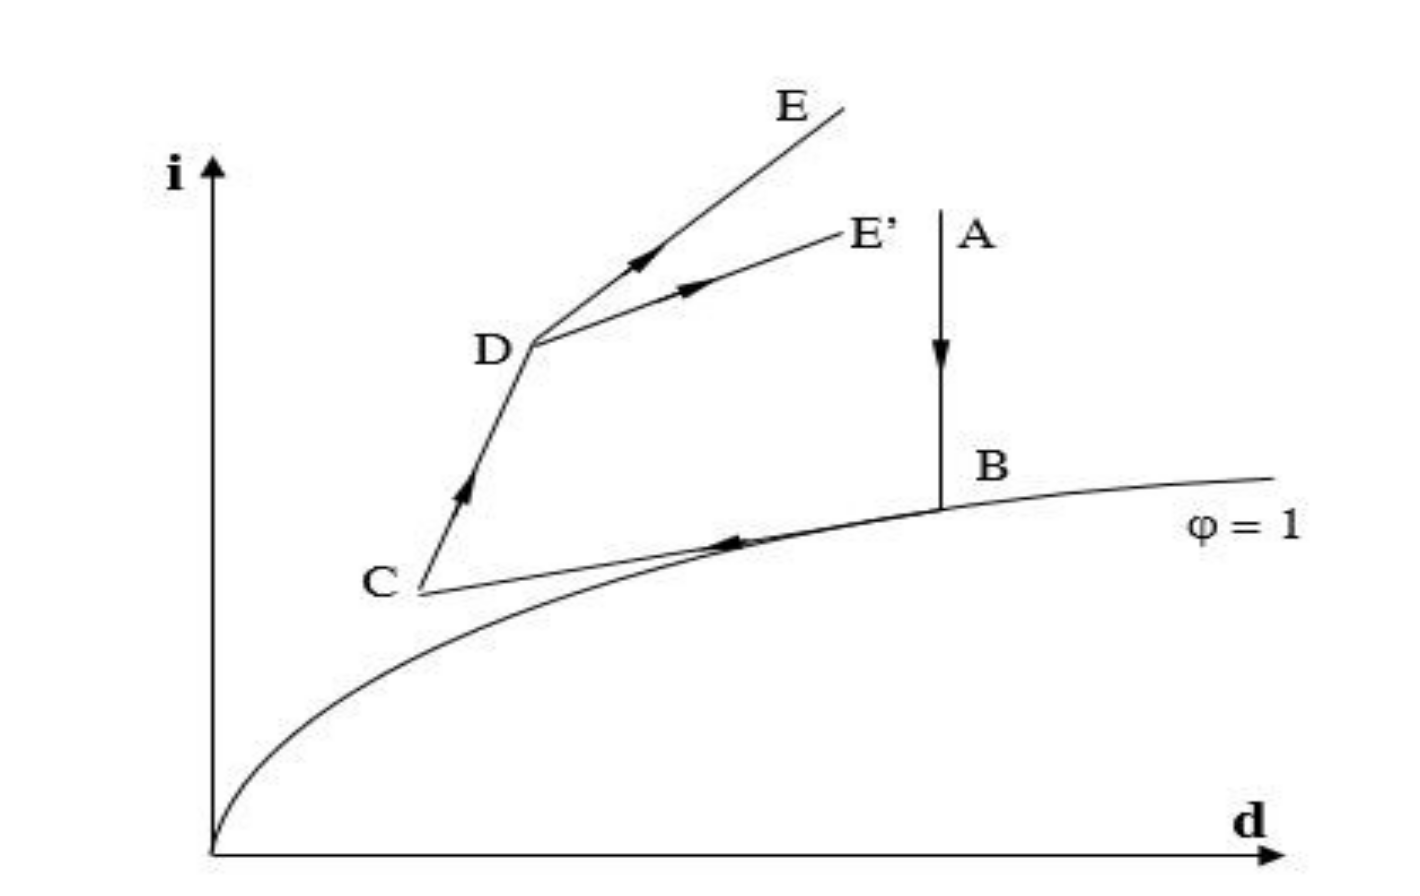
\includegraphics[width=0.75\linewidth]{Images/figure10.png}
    \caption{The diagram of the change in air when traveling through the aerodynamic tube in practice.}
    \label{fig:practice_diagram}
\end{figure}
\begin{itemize}
    \item \textbf{Through the cooler (AB, BC):} At the end of cooling (Point C), the air is not at saturated state as in theory, but at an unsaturated state. This is because the air coming out of the cooler receives extra heat from the surroundings before reaching the thermometer.
    \item \textbf{Through the dryer (CD):} The drying process does not take place at constant $d$ as in theory; in practice $d$ gradually increases. This is because air picks up moisture from the surroundings before reaching the measurement point.
    \item \textbf{Through the steam nozzle (DE):} The change of air state is essentially the same as in theory, because the surroundings do not significantly affect the results.
\end{itemize}

\subsection{Comparisons between theoretical and practical values}
\begin{itemize}
    \item \textbf{Capacity of cooler:} Theoretical capacity is larger than practical capacity because of heat loss to the surroundings, so the cooler cannot achieve its full theoretical load.
    \item \textbf{Condensed water from cooler:}
    \begin{itemize}
        \item In theory: $G_{water} = (0.9 \div 2.0)$ kg/h
        \item In practice: $G'_{water} = (0.3 \div 1.0)$ kg/h
    \end{itemize}
    The difference is due to errors when taking condensed water sample and recording the time.
    \item \textbf{Thermal load of Air dryer:} Practical thermal load is smaller than theoretical thermal load because of heat loss to the surroundings, so the amount of heat air receives is smaller than the amount supplied by the dryer.
\end{itemize}

\subsection{Causes of error between practice and theory}
The reliability of the above results is not high due to many factors:
\begin{itemize}
    \item \textbf{Temperature reading errors:} The temperature values shown on the screen are not stable. They usually vary $\pm 1$--$2^\circ$C.
    \item \textbf{Condensed water measurement errors:} We cannot read accurately the value of the graduated cylinder; the self-error of the graduated cylinder; and the error when we record the time.
    \item \textbf{Equipment errors:} Self-error of equipment; the equipment is not well thermally and humidly insulated; the system is not closed so it is affected by the surroundings; airflow into the equipment is not stable.
    \item \textbf{Calculation errors:} When looking up and rounding the data.
\end{itemize}
